%!TEX root = ./seminarpaper.tex

\chapter{Implemented Functions}

	This chapter gives an overview about all implemented functions. Figure \ref{fig:OverviewProbabilityDistributions} on page \pageref{fig:OverviewProbabilityDistributions} shows all of them.

	\begin{figure}[h]
		\centering
		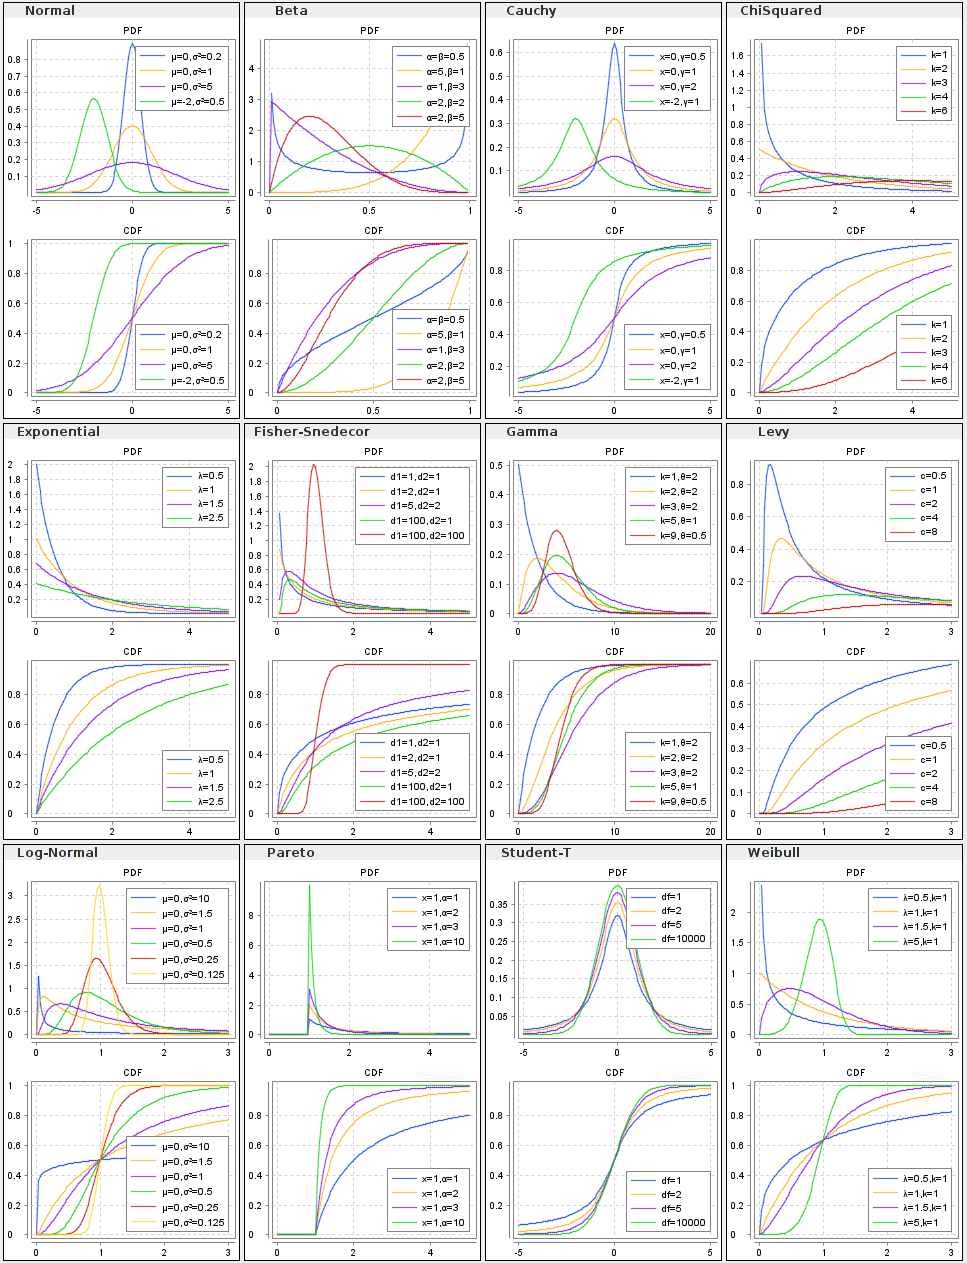
\includegraphics[width=1\textwidth]{Figures/OverviewProbabilityDistributions}~\\
		\caption{Overview Probability Distributions}
		\url{https://commons.apache.org/proper/commons-math/userguide/distribution.html}
		\label{fig:OverviewProbabilityDistributions}
	\end{figure}

	\section{Beta Distribution} \label{sec:beta_distribution}

		The beta distribution has two parameters $\alpha > 0$ and $\beta > 0$ and is defined on the interval $[0,1]$. The \ac{PDF} of the beta distribution is defined as

		$$f(x) = \frac{x^{\alpha-1}(1-x)^{\beta-1}}{B(\alpha,\beta)}  \hspace{.3in} 0 \le x \le 1; \alpha, \beta > 0$$
		\\[0.3cm]		
		with the beta function $B$ as a normalization constant to ensure that the total probability integrates to 1. The formula of the beta function is defined as

		$$B(\alpha,\beta) = \frac{\Gamma(\alpha)\Gamma(\beta)}{\Gamma(\alpha + \beta)}$$
		\\[0.3cm]
		where $\Gamma$ denotes the gamma function. The \ac{CDF} of the beta distribution is defined as

		$$F(x) = I_{x}(\alpha,\beta) = \frac{\int_{0}^{x}{t^{\alpha-1}(1-t)^{\beta-1}dt}}{B(\alpha,\beta)} \hspace{.3in} 0 \le x \le 1; \alpha, \beta > 0$$


	\section{Cauchy Distribution}

		The Cauchy distribution has a location parameter $t$ and a scale parameter $s$ where $s > 0$. The \ac{PDF} of the distribution is defined as

		$$\ds f(x) = \frac{1}{\pi} \cdot \frac{s}{s^2 + (x-t)^2} \quad \hspace{.3in} -\infty<x<\infty$$
		\\[0.3cm]
		The \ac{CDF} is defined as 

		$$\ds F(x) = \frac{1}{2} + \frac{1}{\pi} \cdot \arctan\left(\frac{x-t}{s}\right)$$		

	\section{Chi-squared Distribution}

		The chi-squared distribution (also $\chi^2$-distribution) has only one parameter $k$, where $k \in \mathbb{N}_{>0}$. The \ac{PDF} is defined as

		$$f(x;\,k) =
		\begin{cases}
			\dfrac{x^{(k/2-1)} e^{-x/2}}{2^{k/2} \Gamma\left(\frac k 2 \right)},  & x > 0; \\ 0, & \text{otherwise}.
		\end{cases}$$
		\\[0.3cm]
		where $\Gamma$ is the gamma function. The \ac{CDF} is defined as

		$$F(x;\,k) = \frac{\gamma(\frac{k}{2},\,\frac{x}{2})}{\Gamma(\frac{k}{2})} = P\left(\frac{k}{2},\,\frac{x}{2}\right)$$


	\section{Exponential Distribution}

		The exponential distribution has only the parameter $\lambda$, where $\lambda > 0$. The \ac{PDF} is defined as

		$$f(x;\lambda) = \begin{cases} \lambda e^{-\lambda x} & x \ge 0, \\ 0 & x < 0. \end{cases}$$
		\\[0.3cm]
		The \ac{CDF} is defined as

		$$F(x;\lambda) = \begin{cases} 1-e^{-\lambda x} & x \ge 0 \\ 0 & x < 0. \end{cases}$$

	\section{Fisher-Snedecor Distribution} 

		The Fisher-Snedecor, or F-distribution, has the two parameters $a$ and $b$, where $a,b \in \mathbb{N}_{>0}$. The \ac{PDF} is defined as

		$$
			f(x) = \frac{1}{\mathrm{B}\!\left(\frac{a}{2},\frac{b}{2}\right)} \left(\frac{a}{b}\right)^{\frac{a}{2}} x^{\frac{a}{2} - 1} \left(1+\frac{a}{b}\,x\right)^{-\frac{a+b}{2}}
		$$
		\\[0.3cm]
		where $\Gamma$ denotes the gamma function.
		The \ac{CDF} is defined as

		$$F(x; a,b)=I_{\frac{a x}{a x + b}}\left (\tfrac{a}{2}, \tfrac{b}{2} \right)$$
		\\[0.3cm]
		where $I$ is the regularized incomplete beta function (see section \ref{sec:beta_distribution}).

	\section{Gamma Distribution}

		The gamma distribution has the shape and scale parameters $p$ and $b$, where $p,b > 0$. The \ac{PDF} is defined as

		$$f(x;p,b) =  \frac{x^{p-1}e^{-\frac{x}{b}}}{b^p\Gamma(p)} \quad \text{ for } x > 0 \text{ and } p, b > 0.$$
		\\[0.3cm]
		where $\Gamma(p)$ is a complete \href{https://en.wikipedia.org/wiki/Gamma_function}{gamma function}.		The \ac{CDF} is defined as

		$$F(x;p,b) = \int_0^x f(u;p,b)\,du = \frac{\gamma\left(p, \frac{x}{b}\right)}{\Gamma(p)}$$
		\\[0.3cm]
		where $\gamma\left(p, \frac{x}{b}\right)$ is the lower \href{https://en.wikipedia.org/wiki/Incomplete_gamma_function}{incomplete gamma function}.

	\section{Levy Distribution}

	\section{Log-Normal Distribution}

	\section{Normal Distribution}

	\section{Pareto Distribution}

	\section{Student-T Distribution}
	
		The student distribution has one parameter \nu\ (degrees of freedom) $>$ 0. The \ac{PDF} of the student distribution is defined as
		\\
		$$f(t) = \frac{\Gamma(\frac{\nu+1}{2})} {\sqrt{\nu\pi}\,\Gamma(\frac{\nu}{2})} \left(1+\frac{t^2}{\nu} \right)^{\!-\frac{\nu+1}{2}}$$
		\\
		where $\Gamma$ is the gamma function. The \ac{CDF} of the student distribution can be written in terms of $I$, the regularized incomplete beta function. For $t > 0$
		\\
		$$F(t) = \int_{-\infty}^t f(u)\,du = 1 - \tfrac{1}{2} I_{x(t)}\left(\tfrac{\nu}{2}, \tfrac{1}{2}\right)$$
		\\
		where $$x(t) = \frac{\nu}{{t^2+\nu}}$$

	\section{Weibull Distribution}
	
		The weibull distribution has two parameters $k$ (shape) $>$ 0 and $\gamma$ (scale) $>$ 0 and is defined for \textit{x} \geq\ 0. The \ac{PDF} of the weibull distribution is defined as
		\\
		$$f(x) = \left(\frac{k}{\gamma}\right)\left(\frac{x}{\gamma}\right)^{k-1}e^{-\left(\frac{x}{\gamma}\right)^{k}} \hspace{.3in} x \geq 0; k,\gamma > 0\\$$
		\\
		The \ac{CDF} of the weibull distribution is defined as
		\\
		$$F(x) = 1 - e^{-(x^{\gamma})} \hspace{.3in} x \geq 0; \gamma > 0$$